%!TEX root = ../thesis.tex
% ******************************* Thesis Appendix A ****************************

\chapter{}

\ifpdf
\graphicspath{{chapter-optimisation/Figs/Raster/}{chapter-electroweak/Figs/PDF/}{chapter-optimisation/Figs/}}
\else
\graphicspath{{chapter-optimisation/Figs/Vector/}{chapter-electroweak/Figs/}}
\fi


\section{Additional information on signal region optimisation}\label{app:n-1_plots_cut_opt}

The following figures provide additional information on the signal region optimisation performed in~\cref{ch:signal_region_optimisation}. \Cref{fig:results_z_vs_eff_rest} shows the results of the $N$-dimensional cut scan for the remaining benchmark signal points considered. As before, three different uncertainty configurations are used for computing the significance $Z_\mathrm{B}$, and all values are computed for the two statistically independent subsets used during the $N$-dimensional scan. This approach allows to gauge the impact of statistical fluctuations on the cut combinations tested.

By choosing a well-performing cut combination for each benchmark point, the optimised selections in~\cref{fig:results_n1_800_0,fig:results_n1_800_150,fig:results_n1_800_250,fig:results_n1_600_300,fig:results_n1_400_200,fig:results_n1_300_150} are found after a round of $N-1$ plots. As discussed in~\cref{sec:towards_signal_regions} the optimal cut combinations for each benchmark signal point are consolidated into multiple signal regions designed to be sensitive to different kinematic regions of the model parameter space. 

\Cref{fig:results_HF_scan_app} shows additional information on some of the investigated simplified shape-fit configurations. Two-dimensional shape-fits in $(\mt,\mbb)$, $(\mt,\met)$ and $(\mt,\mct)$ with $3\times 3$ bins each are compared. The configuration using bins in $\mt$ and $\mct$ results in the best expected CL$_s$ values throughout the entire signal grid. Adding a requirement on high values of $\mlb$ to SR-HM further increases the expected sensitivity. Overall, the expected sensitivity achieved through introduction of the two-dimensional shape fit significantly exceeds the sensitivity of the previous analysis iteration (using a one-dimensional shape-fit in $\mt$, scaled to \onethirtynineifb).

\begin{figure}[hb]
	\centering
	\begin{subfigure}[b]{0.5\linewidth}
		\centering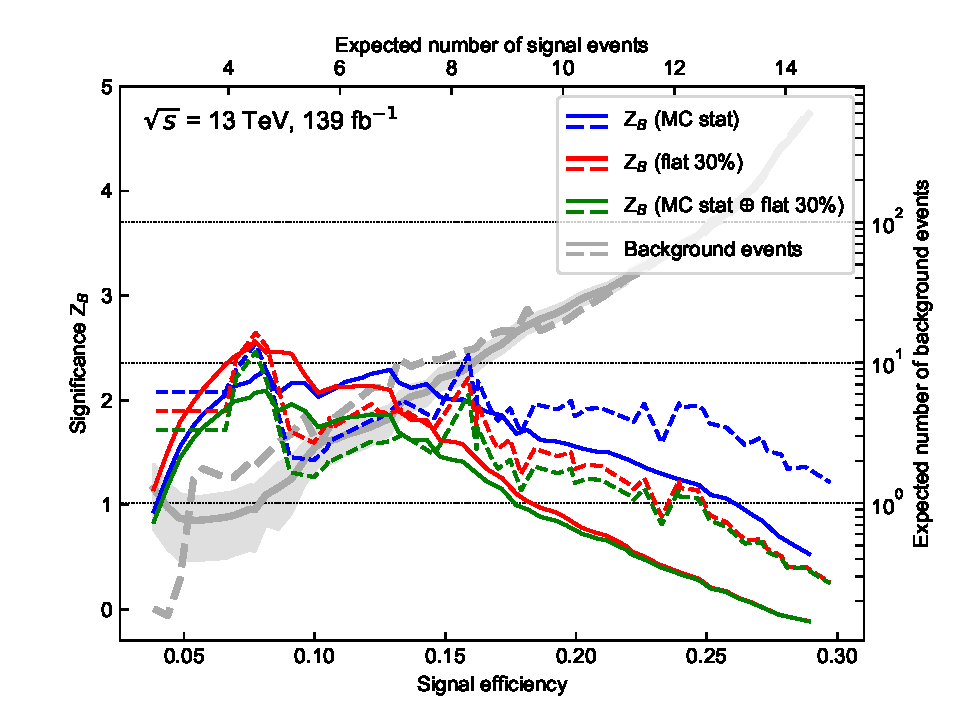
\includegraphics[width=1.0\textwidth]{N-1_cut_scan/z_vs_effs_800_150.pdf}
		\caption{$m(\charg/\neutr), m(\lsp) =  800, \SI{150}{\GeV}$}
	\end{subfigure}\hfill
	\begin{subfigure}[b]{0.5\linewidth}
		\centering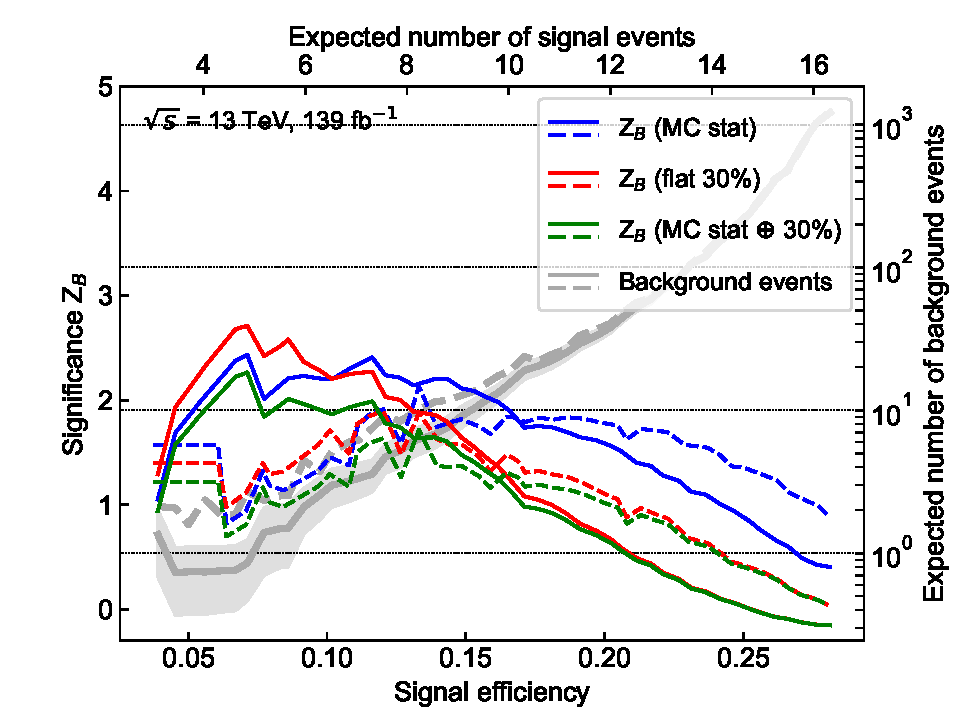
\includegraphics[width=1.0\textwidth]{N-1_cut_scan/z_vs_effs_800_0.pdf}
		\caption{$m(\charg/\neutr), m(\lsp) =  800, \SI{0}{\GeV}$}
	\end{subfigure}\hfill
	\begin{subfigure}[b]{0.5\linewidth}
		\centering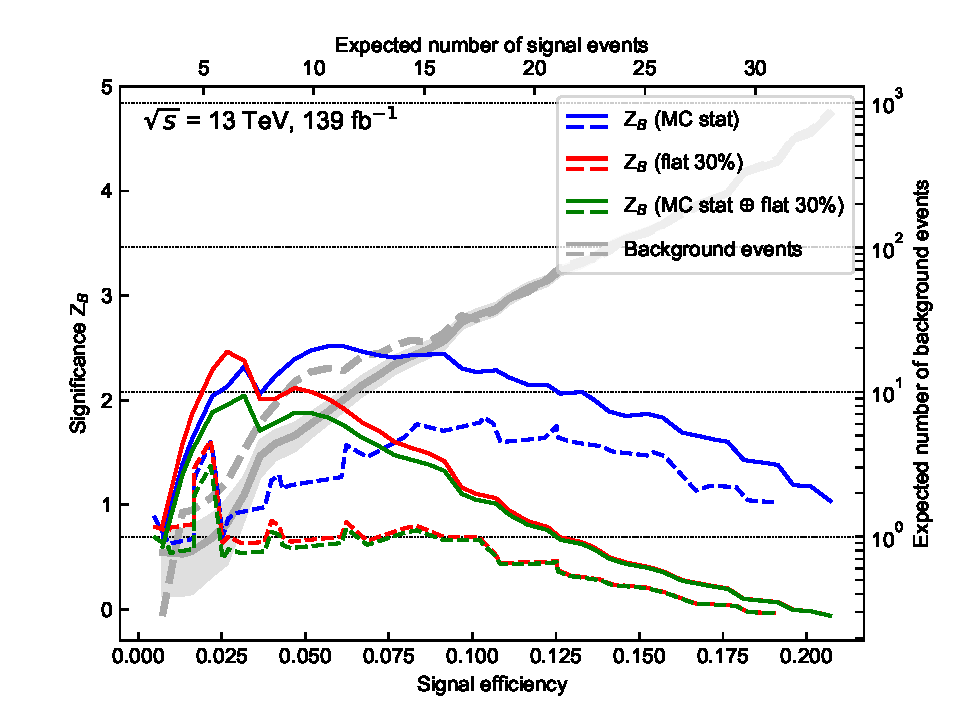
\includegraphics[width=1.0\textwidth]{N-1_cut_scan/z_vs_effs_600_300.pdf}
		\caption{$m(\charg/\neutr), m(\lsp) =  600, \SI{300}{\GeV}$}
	\end{subfigure}\hfill
	\begin{subfigure}[b]{0.5\linewidth}
		\centering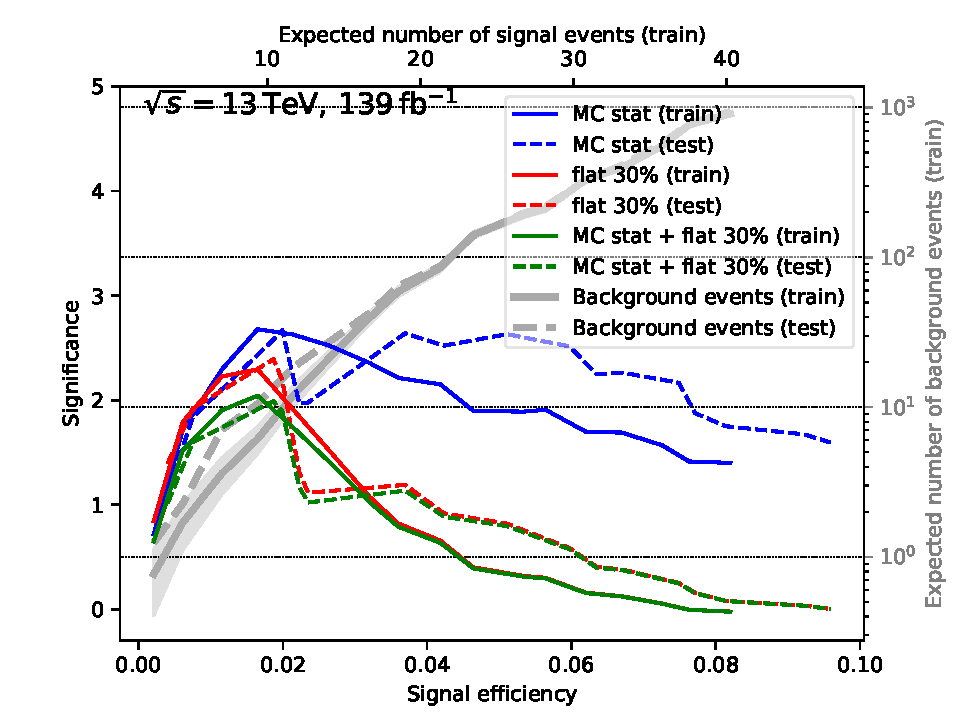
\includegraphics[width=1.0\textwidth]{N-1_cut_scan/z_vs_effs_400_200.pdf}
		\caption{$m(\charg/\neutr), m(\lsp) =  400, \SI{200}{\GeV}$}
	\end{subfigure}\hfill

	\caption[N-dimensional cut scan results]{Results of the $N$-dimensional cut scan for the remaining four benchmark points. The binomial discovery significance $Z_\mathrm{B}$ is plotted against the signal efficiency for varying uncertainty configurations. Additionally, the expected \gls{sm} background rates are shown, including statistical uncertainty for one of the two statistically independent samples (shaded area). The solid and dashed lines represent the two statistically independent subset that the \gls{mc} samples are split into.}
	\label{fig:results_z_vs_eff_rest}
\end{figure}


\begin{figure}
	\centering
	\begin{subfigure}[b]{0.5\linewidth}
		\centering\includegraphics[width=0.9\textwidth]{N-1_cut_scan/n1_800_0/mt}
	\end{subfigure}\hfill
	\begin{subfigure}[b]{0.5\linewidth}
		\centering\includegraphics[width=0.9\textwidth]{N-1_cut_scan/n1_800_0/mct}
	\end{subfigure}\hfill
	\begin{subfigure}[b]{0.5\linewidth}
		\centering\includegraphics[width=0.9\textwidth]{N-1_cut_scan/n1_800_0/met}
	\end{subfigure}\hfill
	\begin{subfigure}[b]{0.5\linewidth}
		\centering\includegraphics[width=0.9\textwidth]{N-1_cut_scan/n1_800_0/mlb1}
	\end{subfigure}\hfill
	\begin{subfigure}[b]{0.5\linewidth}
		\centering\includegraphics[width=0.9\textwidth]{N-1_cut_scan/n1_800_0/mbb_both}
	\end{subfigure}\hfill
	\begin{subfigure}[b]{0.5\linewidth}
		\centering\includegraphics[width=0.9\textwidth]{N-1_cut_scan/n1_800_0/nJet30}
	\end{subfigure}

	\caption[N-1 plots for the chosen cut combination for the (800, 0) signal point]{N-1 plots for the chosen cut combination for the $(m(\charg/\neutr), m(\lsp)) = (\SI{800}{\GeV}, \SI{0}{\GeV})$ signal point. The shaded region includes \gls{mc} statistical uncertainty as well as 30\% systematic uncertainty (added in quadrature) on the background. The significance is computed using the binomial discovery significance using the uncertainty on the background.}
	\label{fig:results_n1_800_0}
\end{figure}



\begin{figure}
	\centering
	\begin{subfigure}[b]{0.5\linewidth}
		\centering\includegraphics[width=0.9\textwidth]{N-1_cut_scan/n1_800_150/mt}
	\end{subfigure}\hfill
	\begin{subfigure}[b]{0.5\linewidth}
		\centering\includegraphics[width=0.9\textwidth]{N-1_cut_scan/n1_800_150/mct}
	\end{subfigure}\hfill
	\begin{subfigure}[b]{0.5\linewidth}
		\centering\includegraphics[width=0.9\textwidth]{N-1_cut_scan/n1_800_150/met}
	\end{subfigure}\hfill
	\begin{subfigure}[b]{0.5\linewidth}
		\centering\includegraphics[width=0.9\textwidth]{N-1_cut_scan/n1_800_150/mlb1}
	\end{subfigure}\hfill
	\begin{subfigure}[b]{0.5\linewidth}
		\centering\includegraphics[width=0.9\textwidth]{N-1_cut_scan/n1_800_150/mbb_both}
	\end{subfigure}\hfill
	\begin{subfigure}[b]{0.5\linewidth}
		\centering\includegraphics[width=0.9\textwidth]{N-1_cut_scan/n1_800_150/nJet30}
	\end{subfigure}

	\caption[N-1 plots for the chosen cut combination for the (800, 150) signal point]{N-1 plots for the chosen cut combination for the $(m(\charg/\neutr), m(\lsp)) = (\SI{800}{\GeV}, \SI{150}{\GeV})$ signal point. The shaded region includes \gls{mc} statistical uncertainty as well as 30\% systematic uncertainty (added in quadrature) on the background. The significance is computed using the binomial discovery significance using the uncertainty on the background.}
	\label{fig:results_n1_800_150}
\end{figure}

\begin{figure}
	\centering
	\begin{subfigure}[b]{0.5\linewidth}
		\centering\includegraphics[width=0.9\textwidth]{N-1_cut_scan/n1_800_250/mt}
	\end{subfigure}\hfill
	\begin{subfigure}[b]{0.5\linewidth}
		\centering\includegraphics[width=0.9\textwidth]{N-1_cut_scan/n1_800_250/mct}
	\end{subfigure}\hfill
	\begin{subfigure}[b]{0.5\linewidth}
		\centering\includegraphics[width=0.9\textwidth]{N-1_cut_scan/n1_800_250/met}
	\end{subfigure}\hfill
	\begin{subfigure}[b]{0.5\linewidth}
		\centering\includegraphics[width=0.9\textwidth]{N-1_cut_scan/n1_800_250/mlb1}
	\end{subfigure}\hfill
	\begin{subfigure}[b]{0.5\linewidth}
		\centering\includegraphics[width=0.9\textwidth]{N-1_cut_scan/n1_800_250/mbb_both}
	\end{subfigure}\hfill
	\begin{subfigure}[b]{0.5\linewidth}
		\centering\includegraphics[width=0.9\textwidth]{N-1_cut_scan/n1_800_250/nJet30}
	\end{subfigure}

	\caption[N-1 plots for the chosen cut combination for the (800, 250) signal point]{N-1 plots for the chosen cut combination for the $(m(\charg/\neutr), m(\lsp)) = (\SI{800}{\GeV}, \SI{250}{\GeV})$ signal point. The shaded region includes \gls{mc} statistical uncertainty as well as 30\% systematic uncertainty (added in quadrature) on the background. The significance is computed using the binomial discovery significance using the uncertainty on the background.}
	\label{fig:results_n1_800_250}
\end{figure}

\begin{figure}
	\centering
	\begin{subfigure}[b]{0.5\linewidth}
		\centering\includegraphics[width=0.9\textwidth]{N-1_cut_scan/n1_600_300/mt}
	\end{subfigure}\hfill
	\begin{subfigure}[b]{0.5\linewidth}
		\centering\includegraphics[width=0.9\textwidth]{N-1_cut_scan/n1_600_300/mct}
	\end{subfigure}\hfill
	\begin{subfigure}[b]{0.5\linewidth}
		\centering\includegraphics[width=0.9\textwidth]{N-1_cut_scan/n1_600_300/met}
	\end{subfigure}\hfill
	\begin{subfigure}[b]{0.5\linewidth}
		\centering\includegraphics[width=0.9\textwidth]{N-1_cut_scan/n1_600_300/mlb1}
	\end{subfigure}\hfill
	\begin{subfigure}[b]{0.5\linewidth}
		\centering\includegraphics[width=0.9\textwidth]{N-1_cut_scan/n1_600_300/mbb_both}
	\end{subfigure}\hfill
	\begin{subfigure}[b]{0.5\linewidth}
		\centering\includegraphics[width=0.9\textwidth]{N-1_cut_scan/n1_600_300/nJet30}
	\end{subfigure}

	\caption[N-1 plots for the chosen cut combination for the (600, 300) signal point]{N-1 plots for the chosen cut combination for the $(m(\charg/\neutr), m(\lsp)) = (\SI{600}{\GeV}, \SI{300}{\GeV})$ signal point. The shaded region includes \gls{mc} statistical uncertainty as well as 30\% systematic uncertainty (added in quadrature) on the background. The significance is computed using the binomial discovery significance using the uncertainty on the background.}
	\label{fig:results_n1_600_300}
\end{figure}

\begin{figure}
	\centering
	\begin{subfigure}[b]{0.5\linewidth}
		\centering\includegraphics[width=0.9\textwidth]{N-1_cut_scan/n1_400_200/mt}
	\end{subfigure}\hfill
	\begin{subfigure}[b]{0.5\linewidth}
		\centering\includegraphics[width=0.9\textwidth]{N-1_cut_scan/n1_400_200/mct}
	\end{subfigure}\hfill
	\begin{subfigure}[b]{0.5\linewidth}
		\centering\includegraphics[width=0.9\textwidth]{N-1_cut_scan/n1_400_200/met}
	\end{subfigure}\hfill
	\begin{subfigure}[b]{0.5\linewidth}
		\centering\includegraphics[width=0.9\textwidth]{N-1_cut_scan/n1_400_200/mlb1}
	\end{subfigure}\hfill
	\begin{subfigure}[b]{0.5\linewidth}
		\centering\includegraphics[width=0.9\textwidth]{N-1_cut_scan/n1_400_200/mbb_both}
	\end{subfigure}\hfill
	\begin{subfigure}[b]{0.5\linewidth}
		\centering\includegraphics[width=0.9\textwidth]{N-1_cut_scan/n1_400_200/nJet30}
	\end{subfigure}

	\caption[N-1 plots for the chosen cut combination for the (400, 200) signal point]{N-1 plots for the chosen cut combination for the $(m(\charg/\neutr), m(\lsp)) = (\SI{400}{\GeV}, \SI{200}{\GeV})$ signal point. The shaded region includes \gls{mc} statistical uncertainty as well as 30\% systematic uncertainty (added in quadrature) on the background. The significance is computed using the binomial discovery significance using the uncertainty on the background.}
	\label{fig:results_n1_400_200}
\end{figure}

\begin{figure}
	\centering
	\begin{subfigure}[b]{0.5\linewidth}
		\centering\includegraphics[width=0.9\textwidth]{N-1_cut_scan/n1_300_150/mt}
	\end{subfigure}\hfill
	\begin{subfigure}[b]{0.5\linewidth}
		\centering\includegraphics[width=0.9\textwidth]{N-1_cut_scan/n1_300_150/mct}
	\end{subfigure}\hfill
	\begin{subfigure}[b]{0.5\linewidth}
		\centering\includegraphics[width=0.9\textwidth]{N-1_cut_scan/n1_300_150/met}
	\end{subfigure}\hfill
	\begin{subfigure}[b]{0.5\linewidth}
		\centering\includegraphics[width=0.9\textwidth]{N-1_cut_scan/n1_300_150/mlb1}
	\end{subfigure}\hfill
	\begin{subfigure}[b]{0.5\linewidth}
		\centering\includegraphics[width=0.9\textwidth]{N-1_cut_scan/n1_300_150/mbb_both}
	\end{subfigure}\hfill
	\begin{subfigure}[b]{0.5\linewidth}
		\centering\includegraphics[width=0.9\textwidth]{N-1_cut_scan/n1_300_150/nJet30}
	\end{subfigure}

	\caption[N-1 plots for the chosen cut combination for the (300, 150) signal point]{N-1 plots for the chosen cut combination for the $(m(\charg/\neutr), m(\lsp)) = (\SI{300}{\GeV}, \SI{150}{\GeV})$ signal point. The shaded region includes \gls{mc} statistical uncertainty as well as 30\% systematic uncertainty (added in quadrature) on the background. The significance is computed using the binomial discovery significance using the uncertainty on the background.}
	\label{fig:results_n1_300_150}
\end{figure}


\begin{figure}
	\centering
	\begin{subfigure}[b]{0.5\linewidth}
		\centering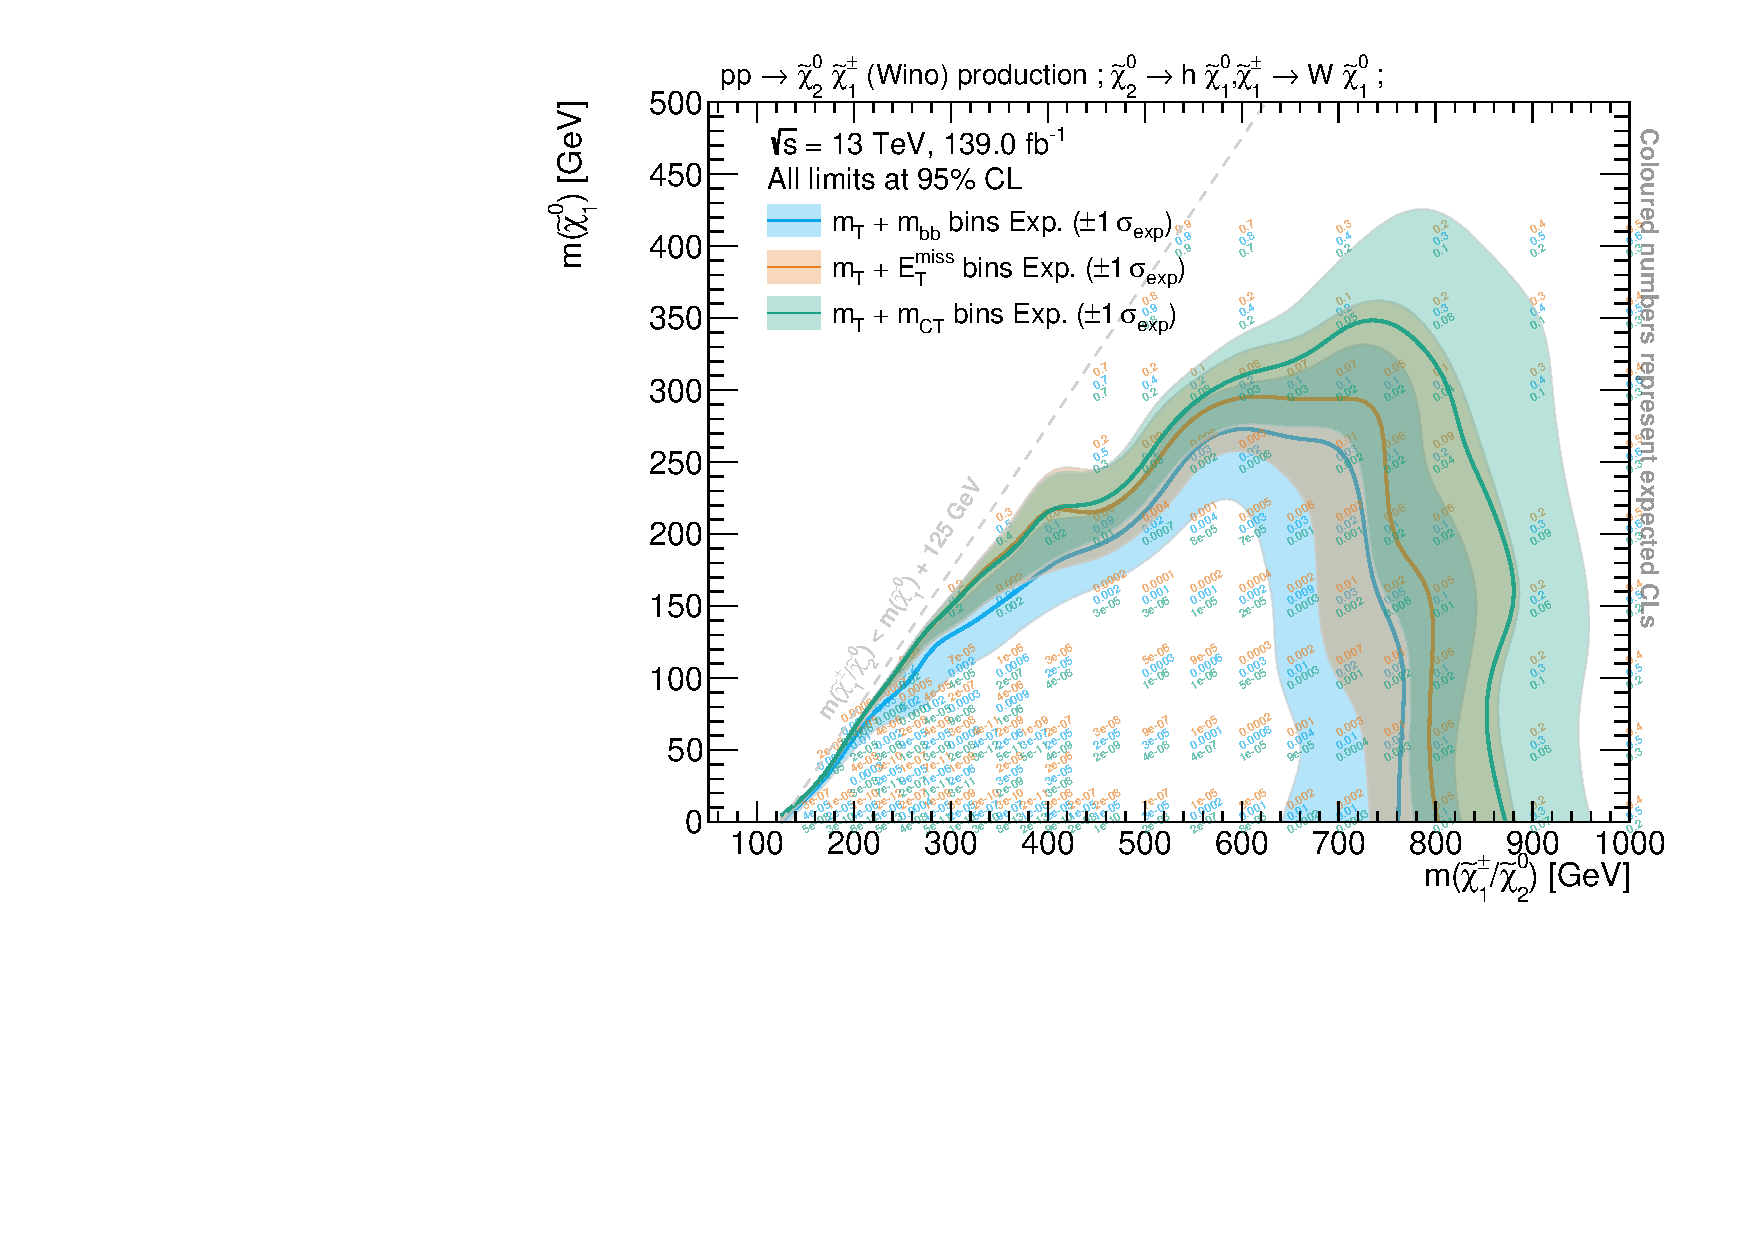
\includegraphics[width=1.0\textwidth]{HF/plot_binnings_cls}
		\caption{\label{fig:plot_binnings_cls}}
	\end{subfigure}\hfill
	\begin{subfigure}[b]{0.5\linewidth}
		\centering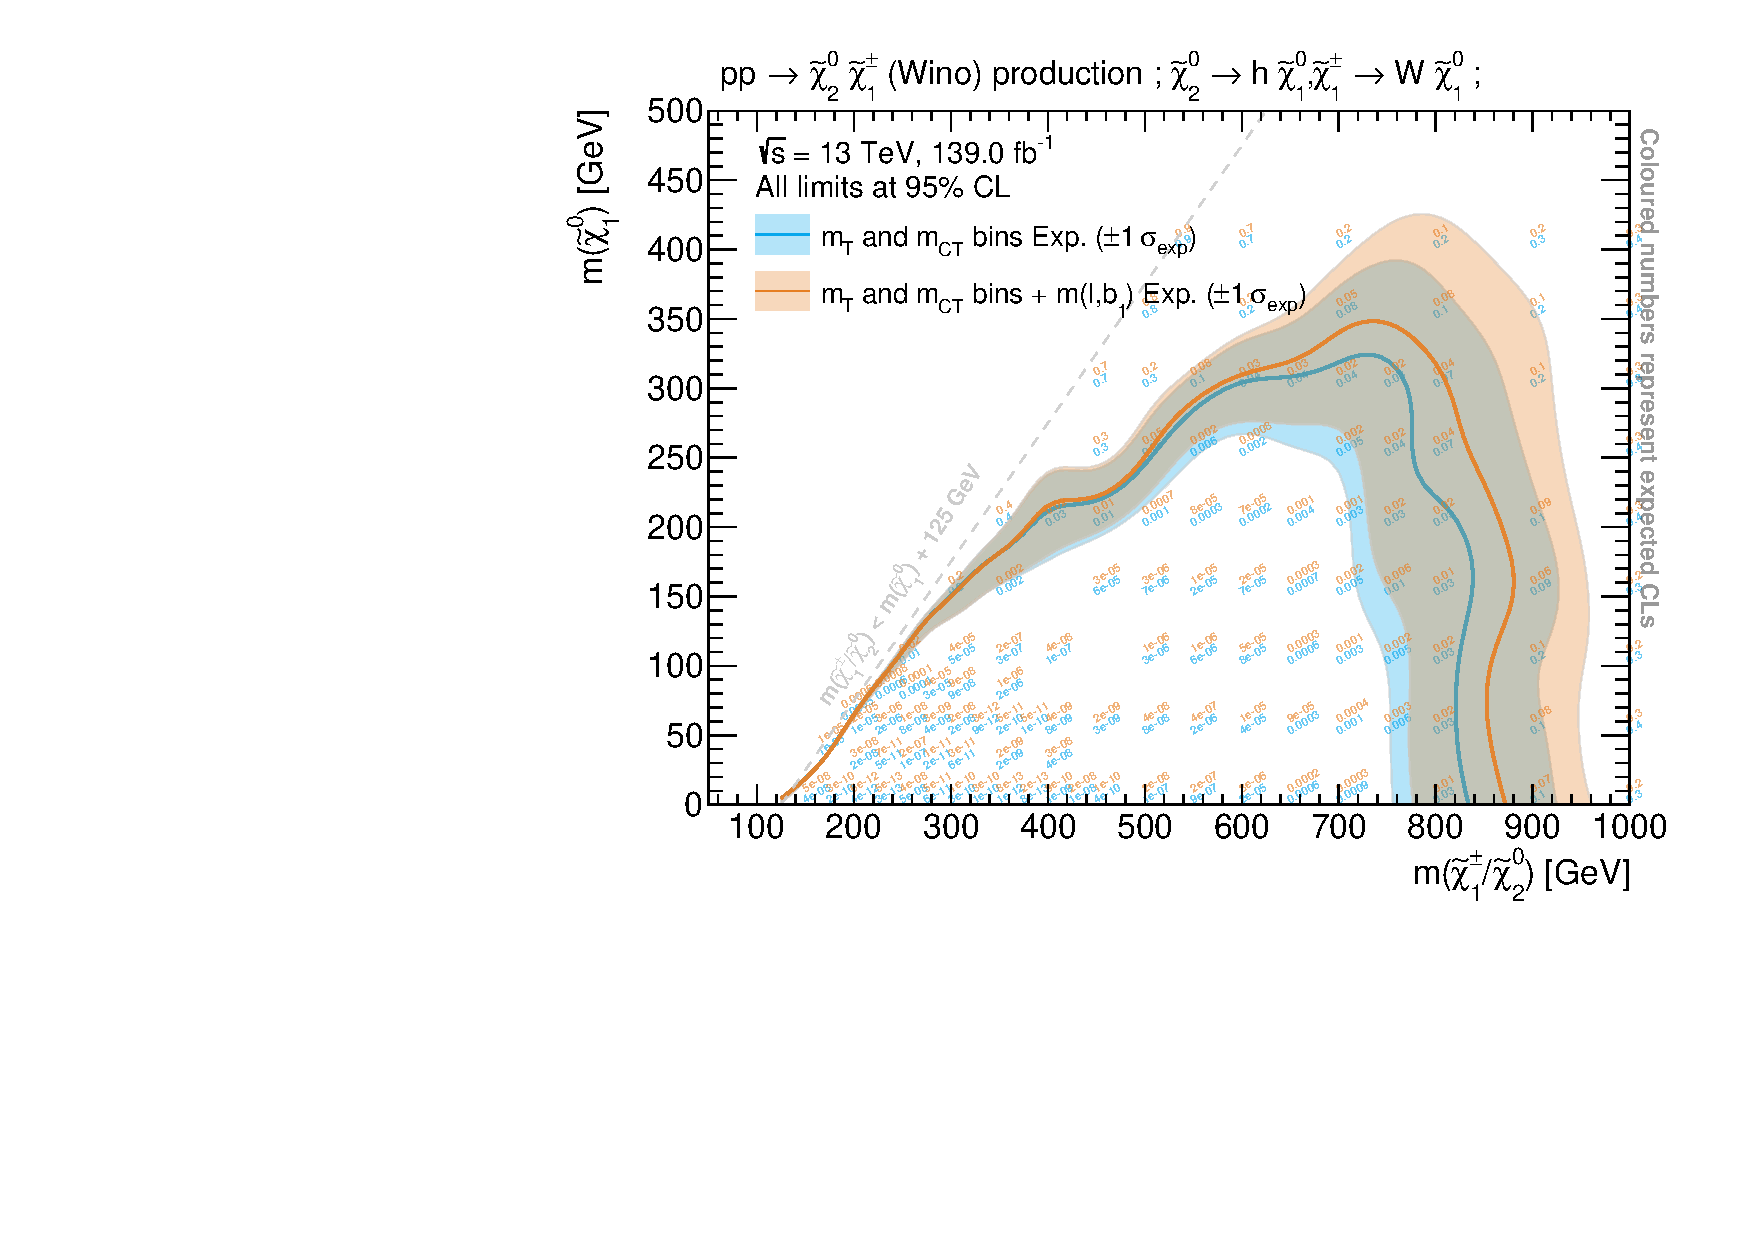
\includegraphics[width=1.0\textwidth]{HF/plot_mlb1_cls}
		\caption{\label{fig:plot_mlb1_cls}}
	\end{subfigure}\hfill
	\begin{subfigure}[b]{0.5\linewidth}
		\centering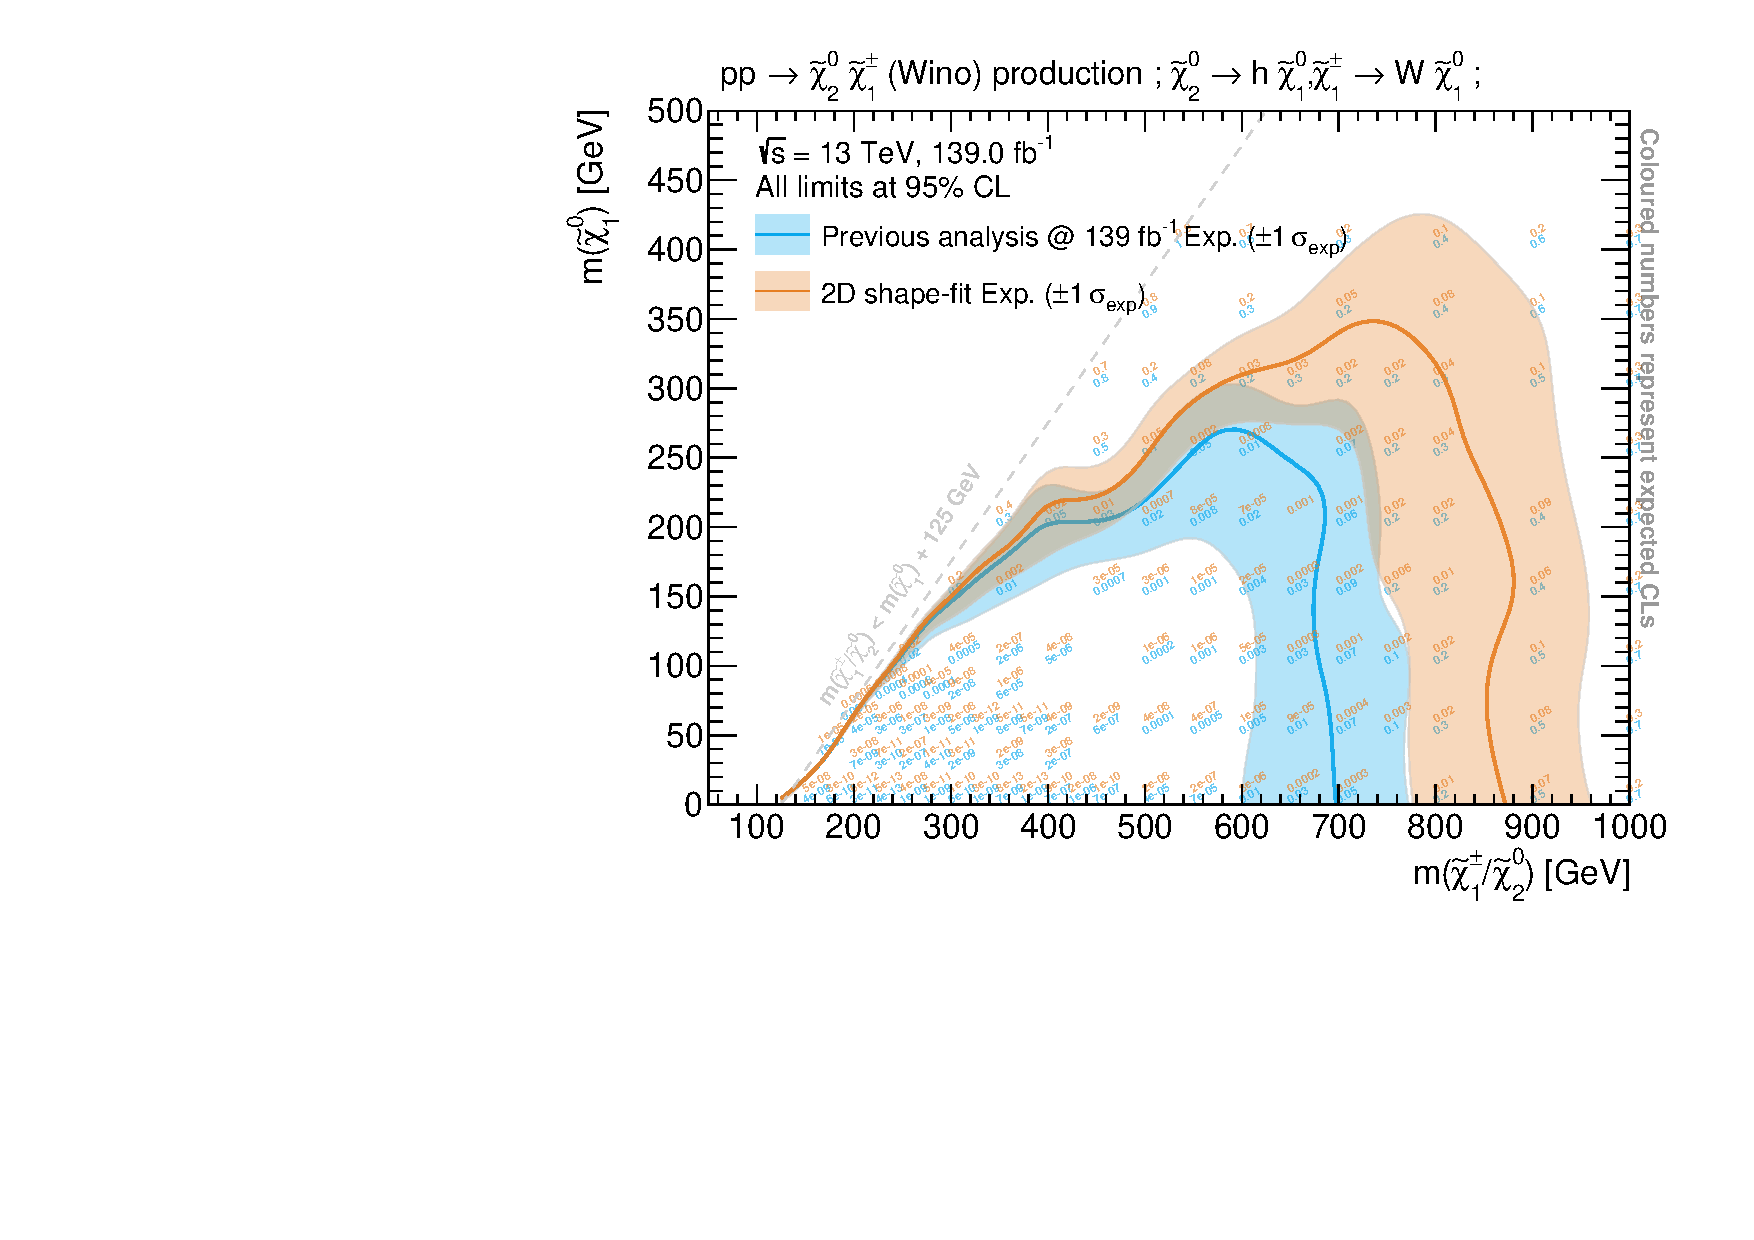
\includegraphics[width=1.0\textwidth]{HF/plot_2d_shapefit_cls}
		\caption{\label{fig:plot_2d_shapefit_cls}}
	\end{subfigure}\hfill

	\caption{Comparison of different shape-fit configurations. Fig.~\subref{fig:plot_binnings_cls} compares three different two-dimensional shape-fit configurations using $3\times 3$ bins in ($\mt$, $\etmiss$), ($\mt$, $\mbb$) and ($\mt$, $\mct$). Fig.~\subref{fig:plot_mlb1_cls} illustrates the sensitivity increase achieved through a requirement on high $\mlb$ values in SR-HM on top of the two-dimensional shape-fit in $\mt$ and $\mct$. Fig.~\subref{fig:plot_2d_shapefit_cls} compares the two-dimensional shape-fit in $\mt$ and $\mct$ to the previous analysis iteration signal regions scaled to \onethirtynineifb. All shown exclusion limits are expected limits at 95\% CL, using \gls{mc} statistical and 30\% systematic uncertainty. Background estimation in the signal regions is taken directly from \gls{mc} for all \gls{sm} backgrounds.}
	\label{fig:results_HF_scan_app}
\end{figure}
